\chapter{\ifcpe บทนำ\else Introduction\fi}

\section{\ifcpe ที่มาของโครงงาน\else Project rationale\fi}
\label{sec:project_rationale}


การสอบปลายภาคหรือการทดสอบความรู้ในช่วงท้ายของการเรียนเป็นส่วนหนึ่งในการวัดระดับความรู้ที่นักศึกษาได้เรียนรู้ไปในวิชานั้น ๆ 
ซึ่งสามารถบ่งบอกถึงความเข้าใจ เอาใจใส่ของนักศึกษาคนนั้น ๆ ซึ่งปัจจัยที่มีผลต่อการสอบนั้นมีอยู่หลายปัจจัย 
ตัวอย่างเช่น ความตั้งใจ ความพยายาม ความเอาใจใส่กับรายวิชาของนักศึกษา แต่ก็ยังมีปัจจัยอีกหนึ่งปัจจัยที่มีผลต่อการสอบปลายภาคด้วย 
คือตารางสอบปลายภาคของนักศึกษา โดยตารางสอบนั้นอาจจะส่งผลกระทบต่อนักศึกษาหากทางมหาวิทยาลัยมีการจัดตารางสอบไม่ดีพอ 
ซึ่งในที่นี้จะกล่าวถึงการจัดตารางสอบของมหาวิทยาลัยเชียงใหม่ ซึ่งในแต่ละภาคการศึกษานั้นมีนักศึกษาที่เรียนมากกว่า 30,000 คน\CIreply{consistency: มี , หรือไม่} 
มีวิชาที่เปิดให้ลงทะเบียนมากกว่า 3000 วิชา มีคู่วิชาที่มีนักศึกษาลงทะเบียนพร้อมกันอย่างน้อย 1 คน มากกว่า 30000 คู่วิชา 
โดยตารางสอบนั้นจะเป็นตารางที่ถูกจัดไว้ก่อนการลงทะเบียนเรียนของนักศึกษา ในการลงทะเบียนเรียน นักศึกษาจะต้องพิจารณาเวลาสอบ และเลือกลงทะเบียนไม่ให้มีวิชาที่สอบตรงกัน 
มิฉะนั้นนักศึกษาจะต้องถอนวิชาใดวิชาหนึ่งที่เวลาสอบตรงกันออก หรือจะได้รับผลการประเมินขั้น F ในวิชาที่ไม่สามารถเข้าสอบปลายภาคได้


ทางมหาวิทยาลัยเชียงใหม่คาดหวังว่านักศึกษาจะเลือกลงทะเบียนเรียนวิชาต่าง ๆ โดยเลือกลงวิชาที่เวลาเรียนไม่ตรงกัน 
ดังนั้น ทางมหาวิทยาลัยจึงจัดตารางสอบของนักศึกษาให้กับวิชาที่มีตอนเดียวก่อน โดยจะอ้างอิงตามช่วงเวลาที่เรียน 
วิชาที่เรียนในวันและเวลาเดียวกันจะถูกจัดให้สอบในช่วงเวลาเดียวกัน (เรียกการจัดสอบแบบนี้ว่า Regular Exam ดังแสดงในรูปที่ \ref{fig:regular_exam}) 
%
\CIreply{ใส่ reference อ้างอิงรูปใน caption}
\begin{figure}
    \centering
    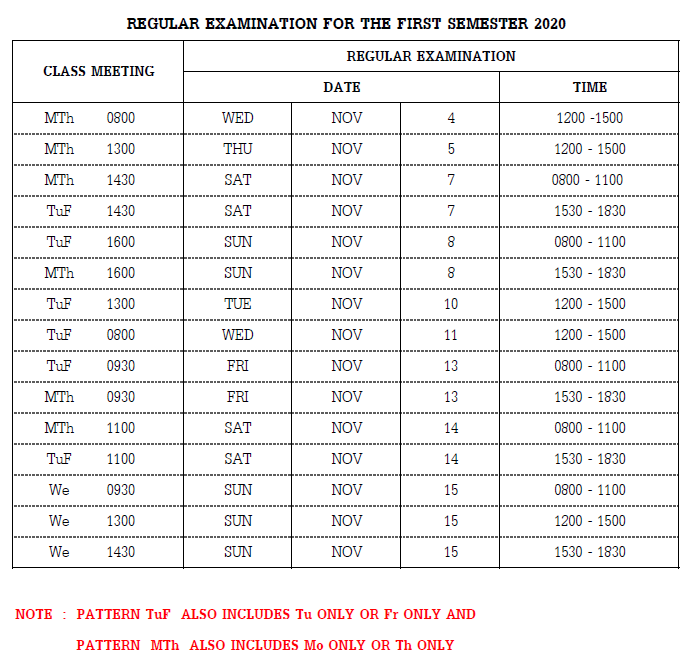
\includegraphics[width=\linewidth]{images/regular_exam.png}
    \caption[ตัวอย่างตารางสอบ regular exam เทอม 1/2563]{ตัวอย่างตารางสอบ regular exam ภาคการศึกษา 1/2563}
    \label{fig:regular_exam}     
\end{figure}
%
ส่วนวิชาที่มีหลายตอน และอาจจะเปิดสอนหลายช่วงเวลา จะถูกจัดให้สอบในช่วงเวลาที่ไม่ตรงกับเวลาสอบของวิชาที่มีตอนเดียว  (เรียกการจัดสอบแบบนี้ว่า Special Exam ดังแสดงในรูปที่ \ref{fig:special_exam}) 
%
\CIreply{ใส่ reference อ้างอิงรูปใน caption}
\begin{figure}
    \centering
    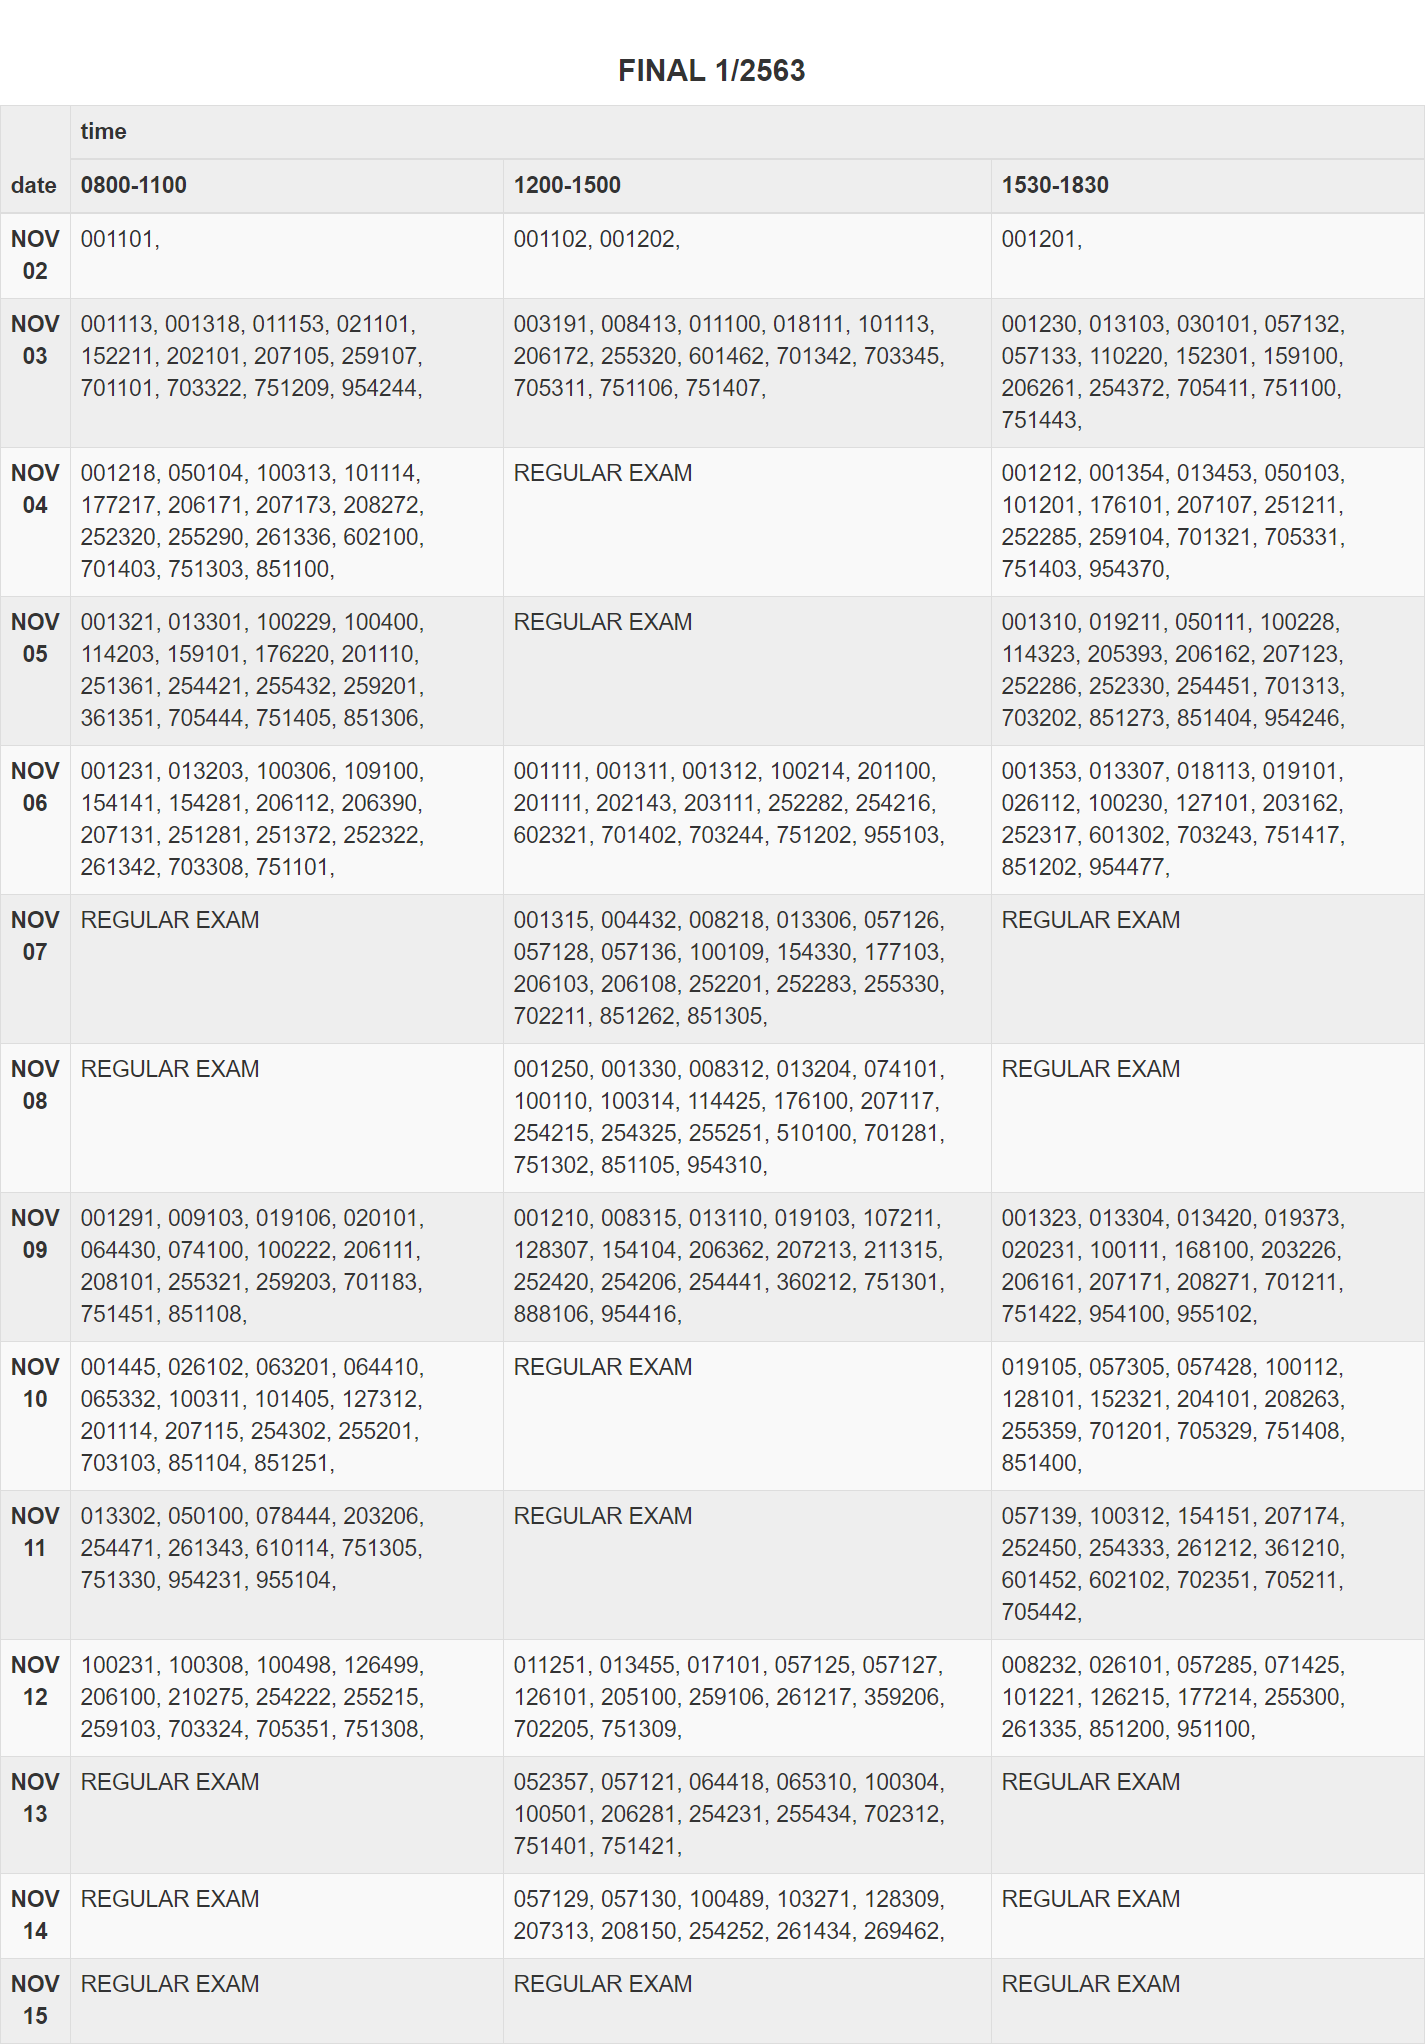
\includegraphics[width=\linewidth]{images/special_exam.png}
    \caption[ตัวอย่างตารางสอบ special exam เทอม 1/2563]{ตัวอย่างตารางสอบ special exam ภาคการศึกษา 1/2563}
    \label{fig:special_exam}     
\end{figure}
เพื่อให้นักศึกษาทั้งหมดที่ลงทะเบียนวิชาเดียวกัน แต่อาจจะคนละตอนกัน สามารถสอบในเวลาเดียวกันได้ เป็นการป้องกันข้อสอบรั่วไหลทางหนึ่ง 
ซึ่งการจัดตารางสอบในลักษณะดังกล่าวนั้นทําให้นักศึกษาไม่สามารถลงทะเบียนวิชาที่สนใจได้อย่างอิสระ เนื่องจากตารางสอบตรงกันหรือเวลาสอบของสองวิชาที่ต้องการลงทะเบียนนั้นติดกันมากเกินไป นอกจากนี้ การจัดตารางสอบด้วยวิธีนี้ ทำให้บางวิชานั้นถูกกําหนดวันสอบให้อยู่ในช่วงท้าย ๆ ของฤดูกาลสอบ 
ทําให้นักศึกษาบางคนมีวันเว้นว่างระหว่างการสอบหลายวันเพราะจําเป็นต้องอยู่รอทำการสอบในวิชาท้าย ๆ ซึ่งปัญหาดังที่กล่าวมานี้ก็อาจเกิดขึ้นกับมหาวิทยาลัยอื่น ๆ ที่มีวิธีการจัดการกับตารางสอบในรูปแบบที่คล้าย ๆ กันนี้เช่นกัน


แม้ว่างานวิจัยของ Ender {\"O}zcan~\cite{fes} จะได้สร้างโปรแกรมสำหรับจัดตารางสอบมาก่อน โดยมีการจัดตารางสอบแบ่งเป็นตารางสอบของวิชาภายในคณะและวิชาภายในภาควิชา 
แต่ก็ไม่สามารถใช้ได้กับวิชาเรียนของทางมหาวิทยาลัยเชียงใหม่ เนื่องจากมีวิชาศึกษาทั่วไป (General Education) ที่มีนักศึกษาจากต่างคณะสามารถลงทะเบียนเรียนร่วมกันได้
\CIreply{หากมีงานอื่นๆ ที่เกี่ยวข้อง เอามาใส่ตรงนี้ ใส่อย่างเดียวดูโดดเดี่ยวไปหน่อย}

จากปัญหาข้างต้น ทีมผู้พัฒนาคาดว่าการพัฒนาระบบจัดตารางสอบโดยใช้ข้อมูลลงทะเบียนของนักศึกษา หลังจากการลงทะเบียนเสร็จสิ้นแล้ว 
จะช่วยให้นักศึกษามีอิสระในการเลือกลงวิชาเรียนมากขึ้น ช่วยลดจำนวนนักศึกษาที่ต้องสอบสองวิชาติดกันในหนึ่งวันให้น้อยลง และลดวันเว้นว่างระหว่างช่วงเวลาสอบ
ซึ่งจะช่วยลดความเครียดส่วนหนึ่งในช่วงสอบของนักศึกษาได้

\section{\ifcpe วัตถุประสงค์ของโครงงาน\else Objectives\fi}
\label{sec:Objectives}
\begin{enumerate}
    \item เพื่อพัฒนาโปรแกรมสำหรับจัดตารางสอบปลายภาคในมหาวิทยาลัย จากข้อมูลการลงทะเบียนของนักศึกษา โดยตารางสอบที่ได้ต้องมีคุณสมบัติดังนี้
    \begin{itemize}
        \item ต้องไม่มีนักศึกษาคนใด ๆ ถูกกำหนดให้สอบสองวิชาในเวลาเดียวกัน
        \item จำนวนนักศึกษาที่มีสอบหลายวิชาติดกันในวันเดียว ลดลงจากตารางสอบดั้งเดิม
        \item จำนวนนักศึกษาที่มีช่วงวันที่เว้นจากการสอบวิชาก่อนหน้ามากกว่า 3 วัน ลดลงจากตารางสอบดั้งเดิม
        \item ในแต่ละช่วงเวลาที่จัดสอบ จำนวนนักศึกษาที่สอบจะต้องไม่เกินจำนวนที่นั่งสอบที่ทางมหาวิทยาลัยสามารถจัดให้ได้
    \end{itemize}
    \item เพื่อขจัดปัญหานักศึกษาไม่สามารถลงทะเบียนในรายวิชาที่ต้องการได้อย่างอิสระ เนื่องจากตารางสอบของรายวิชาที่ต้องการลงทะเบียนถูกจัดไว้ล่วงหน้าให้สอบในช่วงเวลาเดียวกัน
\end{enumerate}

\section{\ifcpe ขอบเขตของโครงงาน\else Project scope\fi}
เป้าหมายของโครงงานนี้ ต้องการพัฒนาโปรแกรมสำหรับจัดตารางสอบปลายภาคในระดับมหาวิทยาลัย
โดยโครงงานนี้จะพิจารณาความต้องการและข้อจำกัดต่าง ๆ ที่ใช้ในการจัดตารางสอบของมหาวิทยาลัยเชียงใหม่
และจะพิจารณาเฉพาะข้อจำกัดทางด้านเวลาเท่านั้น โดยมีขอบเขตของโครงงานดังนี้ 
\subsection{\ifcpe ขอบเขตด้านฮาร์ดแวร์\else Hardware scope\fi}
\begin{enumerate}
    \item ระบบที่จะพัฒนานั้นจะสามารถทำงานได้บนคอมพิวเตอร์ที่ใช้ระบบปฏิบัติการ Windows 7 / Windows 10 หรือระบบปฏิบัติการ Linux เท่านั้น
\end{enumerate}
\subsection{\ifcpe ขอบเขตด้านซอฟต์แวร์\else Software scope\fi}
\begin{enumerate}
    \item ระบบที่จะพัฒนานั้นจะสามารถทำงานได้หากติดตั้ง Python 3.7 ขึ้นไป เท่านั้น \TSNAreply{ไม่แน่ใจ ใส่ไว้ก่อน}
\end{enumerate}
\subsection{ข้อจำกัดที่นำมาพิจารณาในการจัดตารางสอบ}
\begin{enumerate}
    \item ระยะเวลาที่ใช้ในการจัดสอบปลายภาค คือ 2 สัปดาห์
    \item จำนวนช่วงเวลาที่จัดสอบในแต่ละวัน คือ 3 ช่วงเวลา ได้แก่ 8:00--11:00, 12:00--15:00, 
    และ 15:30--18:30
    \item จำนวนที่นั่งสอบที่มหาวิทยาลัยสามารถจัดให้ได้ในตึกอาคารเรียนรวม
    \item จำนวนที่นั่งสอบในแต่ละห้องสอบของแต่ละคณะ
    \item รายชื่อวิชาเรียนที่มีการจัดสอบปลายภาค
    \item ข้อมูลจากการลงทะเบียนล่วงหน้าและลงทะเบียนรอบปกติ
    \item คู่วิชาเรียนที่มีนักศึกษาลงทะเบียนร่วมกันทั้งสองวิชา โดยคู่วิชาที่มีจำนวนนักศึกษาลงทะเบียนมาก จะมีลำดับความสำคัญสูงกว่า\CIreply{ยังจริงอยู่หรือเปล่า}
\end{enumerate}

\subsection{ข้อจำกัดที่ไม่นำมาพิจารณาในการจัดตารางสอบ}
\begin{enumerate}
    \item การจัดกรรมการคุมสอบให้แต่ละรายวิชา
    \item เวลาเรียนของแต่ละรายวิชา (ซึ่งมีบทบาทสำคัญในการจัดตารางสอบแบบเดิม)
    \item การจัดตารางสอบแยกตามรายวิชาของแต่ละคณะ หรือแต่ละภาควิชา\CIreply{อ่านแล้วยังไม่เคลียร์ว่าจะสื่ออะไร}
    \item ข้อมูลจากการลงทะเบียนเพิ่มเติมหลังกำหนด
\end{enumerate}

\section{\ifcpe ประโยชน์ที่ได้รับ\else Expected outcomes\fi}
\begin{enumerate}
    \item นักศึกษาสามารถเลือกลงทะเบียนวิชาที่ต้องการได้อย่างอิสระ โดยไม่ต้องกังวลว่าวิชาเหล่านั้นจะถูกจัดให้สอบในช่วงเวลาเดียวกัน
    \item ช่วยให้ตารางสอบของนักศึกษาคนใด ๆ มีจำนวนรายวิชาที่ต้องสอบในแต่ละวันน้อยลง
    \item ช่วยลดวันเว้นว่างระหว่างช่วงเวลาสอบของนักศึกษาให้น้อยลง 
\end{enumerate}
\CIreply{อาจจะพูดถึงเรื่องที่นั่งสอบ ที่ไม่ overload ใน regular slot สำหรับ เวลาเรียนที่ prime time}

\section{\ifcpe เทคโนโลยีและเครื่องมือที่ใช้\else Technology and tools\fi}

% \subsection{\ifcpe เทคโนโลยีด้านฮาร์ดแวร์\else Hardware technology\fi}
% \begin{enumerate}

% \end{enumerate}
\subsection{\ifcpe เทคโนโลยีด้านซอฟต์แวร์\else Software technology\fi}
\begin{enumerate}
    \item Visual Studio Code เป็น editor ที่มีไว้สำหรับเขียนและอ่านโค้ดภาษาคอมพิวเตอร์ ซึ่่งสามารถรองรับได้หลายภาษา อีกทั้งยังมีเครื่องมือเสริม(extension)สำหรับอำนวยความสะดวกอีกด้วย โดยเราได้ใช้ visual studio code เขียนระบบอัลกอริทึมและเว็บไซต์สำหรับโปรแกรมจัดตารางสอบปลายภาค
    \item Python เป็นภาษาที่ใช้ในการเขียนโปรแกรมภาษาหนึ่งซึ่งเป็น opensource ทำให้เราสามารถพัฒนาโปรแกรมได้แบบฟรีไม่เสียค่าใช้จ่าย โดยไวยากรณ์ของภาษา python ถูกพัฒนาขึ้นมาโดยมีความตั้งใจว่าจะให้เป็นภาษาที่อ่านง่ายและถูกออกแบบมาให้มีโครงสร้างที่มองเห็นได้โดยไม่ซับซ้อน โดยมักจะใช้คำในภาษาอังกฤษในขณะที่ภาษาอื่นใช้เครื่องหมายวรรคตอน นอกจากนี้ python มีข้อยกเว้นของโครงสร้างทางภาษาน้อยกว่าภาษา c และ pascal โดยเราใช้ภาษาที่เป็นภาษาที่ใช้เขียนอัลกอริทึมต่างๆ รวมทั้งการอ่านข้อมูลและเขียนข้อมูล สำหรับโปรแกรมจัดตารางสอบปลายภาค
    \item Node.js เป็นแพลตฟอร์ม ตัวหนึ่งที่เขียนด้วย javaScript สำหรับเขียนโค้ดของทาง back-end หรือการทำเว็บเซิร์ฟเวอร์ เราใช้ Node.js ในการทำเว็บเซิร์ฟเวอร์ เพื่อเชื่อมต่อทางหน้าเว็บไซต์(front-end)กับฐานข้อมูล 
    \item Vue.js เป็น front-end framework ที่ช่วยให้สามารถเขียน javascript ได้ง่ายขึ้น เขียนสั้นลง ทำให้สามารถลดระยะเวลาในการพัฒนาเว็บไซต์ได้พอสมควร เราได้ใช้ vue.js ในการเพัฒนาเว็บไซต์สำหรับการประเมินอัลกอรึทึมของโปรแกรมจัดตารางสอบปลายภาค
\end{enumerate}
\CIreply{อธิบายเพิ่มเติมคร่าวๆ ว่าแต่ละอย่างใช้เพื่ออะไร}

\section{\ifcpe แผนการดำเนินงาน\else Project plan\fi}

\begin{plan}{7}{2020}{3}{2021}
    \planitem{7}{2020}{10}{2020}{Literature Review}
    \planitem{9}{2020}{10}{2020}{เก็บข้อมูลความคิดเห็นนักศึกษา}
    \planitem{10}{2020}{10}{2020}{เขียนรายงาน}
    \planitem{11}{2020}{12}{2020}{เก็บข้อมูลรายวิชาที่ไม่จัดสอบ}
    \planitem{11}{2020}{12}{2020}{ออกแบบอัลกอริทึม เวอร์ชัน 1}
    \planitem{12}{2020}{12}{2020}{ทดสอบและประเมินผลอัลกอริทึม}
    \planitem{12}{2020}{1}{2021}{เก็บข้อมูลความจุที่นั่งสอบของแต่ละคณะและอาคารส่วนกลาง}
    \planitem{12}{2020}{1}{2021}{ออกแบบอัลกอริทึม เวอร์ชัน 2}
    \planitem{1}{2021}{2}{2021}{ทดสอบและประเมินผลอัลกอริทึม}
    \planitem{2}{2021}{3}{2021}{เก็บข้อมูลความพึงพอใจและความคิดเห็นของนักศึกษา}
    \planitem{2}{2021}{3}{2021}{สรุปผลการพัฒนาโปรแกรม}
    \planitem{3}{2021}{3}{2021}{เขียนรายงานผลการพัฒนาโปรแกรม}
\end{plan}
\CIreply{ความคิดเห็นแต่ละครั้ง ต่างกันอย่างไร}
\CIreply{อธิบายความแตกต่างของ versions 1 \& 2}
\CIreply{อาจจะเขียนเป็นร้อยแก้วก่อนขึ้นตาราง}


\section{\ifcpe บทบาทและความรับผิดชอบ\else Roles and responsibilities\fi}
\begin{itemize}
\item นายกฤษฏิ์ อุปนันท์: รับผิดชอบหน้าที่ในการเก็บรวบรวมและสรุปผลความคิดเห็นและความต้องการของนักศึกษา
จากแบบสำรวจเพื่อนำมาใช้ในการจัดลำดับความสำคัญของตัวชี้วัดที่ใช้ในการประเมินระบบ
\CIreply{update?}
\item นายธนวงศ์ เสนีวงศ์ ณ อยุธยา: รับผิดชอบหน้าที่ในการศึกษาทฤษฎีที่เกี่ยวข้องและอัลกอริทึมที่จำเป็นต้องใช้ในการพัฒนาระบบ
\CIreply{update?}
\end{itemize}

ในส่วนของการออกแบบอัลกอริทึมและเขียนโปรแกรมเพื่อพัฒนาระบบ ทั้งสองคน\CI{จะ}{?}ช่วยกันออกแบบและพัฒนาโดยแบ่งงานกันอย่างเท่าเทียม
\CIreply{update}

\section{\ifcpe%
ผลกระทบด้านสังคม สุขภาพ ความปลอดภัย กฎหมาย และวัฒนธรรม
\else%
Impacts of this project on society, health, safety, legal, and cultural issues
\fi}

% ผลกระทบทางด้านสังคม: 
ระบบที่เป็นผลลัพธ์ของโครงงานนี้จะสามารถใช้เป็นทางเลือกในการจัดการตารางสอบในระดับมหาวิทยาลัยได้
ซึ่งตารางสอบที่ได้จากโปรแกรมนี้จะช่วยให้นักศึกษาสามารถเลือกเรียนวิชาที่ตนเองต้องการได้อย่างอิสระ โดยไม่มีข้อจำกัดด้านตารางสอบ
เหมือนอย่างระบบเดิมที่ใช้อยู่ในปัจจุบัน อีกทั้งหากมีการนำไปประยุกต์ใช้กับการจัดตารางสอบที่อื่นที่คณาจารย์ยังคงต้องจัดตารางสอบด้วยตัวเองอยู่
จะเป็นการช่วยลดภาระการจัดตารางสอบของคณาจารย์ได้
\CIreply{update?}

\CIreply{เพิ่มเติมด้านสุขภาพ ความปลอดภัย ได้อยู่  ไมต้องเขียนแยกประเด็นทีละหัวข้อก็ได้ เขียนรวมๆ ได้เลย}